\iffalse
\documentclass[journal,12pt,twocolumn]{article}
\usepackage{amsmath,amssymb,amsfonts,amsthm}
\usepackage{txfonts}
\usepackage{tkz-euclide} 
\usepackage{listings}
\usepackage{gvv}       
\usepackage[latin1]{inputenc}   
\usepackage{array}  

\begin{document}

\bibliographystyle{IEEEtran}

\vspace{3cm}

\title{}
\author{EE23BTECH11217 - Prajwal M$^{*}$
}
\maketitle
\newpage
\bigskip

\renewcommand{\thefigure}{\theenumi}
\renewcommand{\thetable}{\theenumi}

\section*{Exercise 9.5}
\noindent25) \hspace{2pt} \textbf{Find the sum of the following series up to n terms and obtain the Z-transform:}
$$ 
\frac{1^3}{1} + \frac{1^3 + 2^3}{1 + 3} + \frac{1^3 + 2^3 + 3^3}{1 + 3 + 5} + \ldots$$

\noindent Solution: 
\fi
\begin{table}[h]
    \centering
    \begin{tabular}{|c|c|c|}
    \hline
    	\textbf{Symbol} & \textbf{Description} \\
    \hline
	  $s\brak{n}$ & sum of n terms \\
    \hline
	  $S\brak{z}$ & Z-transform of s(n)\\
    \hline
	  $s_1\brak{n}$ & $\brak{n+1}^{3} * u\brak{n}$\\
    \hline	  
	  $S_1\brak{z}$ & Z-transform of $s_1\brak{n}$\\
    \hline 
	  $s_2\brak{n}$ & $\brak{2n+1} * u\brak{n}$\\
    \hline 
	  $S_2\brak{z}$ & Z-transform of $s_2\brak{n}$\\
    \hline
\end{tabular}

    \caption{Parameters}
    \label{tab: 11.9.5.25.1}
\end{table}

\begin{align}
    s\brak{n} & = \sum_{r=0}^{n}\brak{\frac{\sum_{i=0}^{r} \brak{i+1}^{3}}{\sum_{i=0}^{r} \brak{2i+1}}} \\
    & = \frac{\brak{n+1}^3 * u\brak{n}}{\brak{2n+1} * u\brak{n}} * u\brak{n} \\
    & = \frac{s_1\brak{n}}{s_2\brak{n}} * u\brak{n}\label{9.5.25.1}
\end{align}
\begin{align}
    % s_1\brak{n} & = \sum_{i=0}^{n} \brak{i+1}^{3}\\
    s_1(n) & = \brak{n+1}^{3} * u\brak{n}\\
    s_1\brak{n} & \system{Z} S_1\brak{z}\\
    \brak{n+1}^3 & \system{Z} \frac{1 + 4z^{-1} + z^{-2}}{\brak{1-z^{-1}}^4}\\ 
    S_1\brak{z} & = \brak{\frac{1 + 4z^{-1} + z^{-2}}{\brak{1-z^{-1}}^4}} \brak{\frac{1}{1-z^{-1}}} & \cbrak{|z| > 1}\\
    & = \frac{1}{(1 - z^{-1})^5} + \frac{4 z^{-1}}{(1 - z^{-1})^5} + \frac{z^{-2}}{(1 - z^{-1})^5}
\end{align}
using \eqref{eq:shiftk} and \eqref{eq:11.9.5.26.12}
\begin{align}
    s_1\brak{n} & = \frac{\brak{n + 4} \brak{n + 3} \brak{n + 2} \brak{n + 1}}{24}u\brak{n+4}\notag\\
    & + \frac{\brak{n + 3} \brak{n + 2} \brak{n + 1} n}{6}u\brak{n+3}\notag\\
    & + \frac{\brak{n + 2} \brak{n + 1} n \brak{n - 1}}{24}u\brak{n+2}\\
    & = \frac{\brak{n+2}^2\brak{n+1}^2}{4} & \cbrak{n\geq0}\label{9.5.25.2}
\end{align}
\begin{align}
    % s_2\brak{n} & = \sum_{i=0}^{n} \brak{2i+1}\\
    s_2\brak{n} & = \brak{2n+1} * u\brak{n}\\
    s_2\brak{n} & \system{Z} S_2\brak{z}\\
    2n+1 & \system{Z} \brak{\frac{1 + z^{-1}}{\brak{1-z^{-1}}^2}}\\  
    S_2\brak{z} & = \brak{\frac{1 + z^{-1}}{\brak{1-z^{-1}}^2}} \brak{\frac{1}{1-z^{-1}}} & \cbrak{|z| > 1}\\
    & = \frac{1}{(1 - z^{-1})^3} + \frac{z^{-1}}{(1 - z^{-1})^3}
\end{align}
using \eqref{eq:shiftk} and \eqref{eq:11.9.5.26.10}
\begin{align}
    s_2\brak{n} & = \frac{\brak{n + 2} \brak{n + 1}}{2}u\brak{n+2}\notag\\
    & + \frac{\brak{n + 1} \brak{n} }{2}u\brak{n+1}\\
    & = \brak{n+1}^2 & \cbrak{n\geq0} \label{9.5.25.3}
\end{align}
replacing \eqref{9.5.25.2} and \eqref{9.5.25.3} in \eqref{9.5.25.1}
\begin{align}
    s\brak{n}& = \frac{\brak{n+2}^2}{4} * u\brak{n} \\
    s\brak{n} & \system{Z} S\brak{z} \\
	\frac{\brak{n+2}^2}{4} & \system{Z} \brak{\frac{4 -3z^{-1} + z^{-2}}{4\brak{1-z^{-1}}^3}}\\ 
    S\brak{z} & = \brak{\frac{4 -3z^{-1} + z^{-2}}{4\brak{1-z^{-1}}^3}} \brak{\frac{1}{1-z^{-1}}} & \cbrak{|z|>1}\\
    & = \frac{1}{(1 - z^{-1})^4} - \frac{3z^{-1}}{4(1 - z^{-1})^4}\notag\\
    & + \frac{z^{-2}}{4(1 - z^{-1})^4}\\
    s\brak{n} & = \frac{\brak{n + 3} \brak{n + 2}\brak{n+1}}{6}u\brak{n+3}\notag\\
    & - \frac{\brak{n + 2} \brak{n + 1}\brak{n}}{8}u\brak{n+2}\notag\\
    & + \frac{\brak{n + 1} \brak{n}\brak{n-1}}{24}u\brak{n+1}\\
    & = \brak{1 + \frac{37n}{24} + \frac{5n^2}{8} + \frac{n^3}{12}} u\brak{n} 
\end{align}

\begin{figure}[h!]
   \centering
   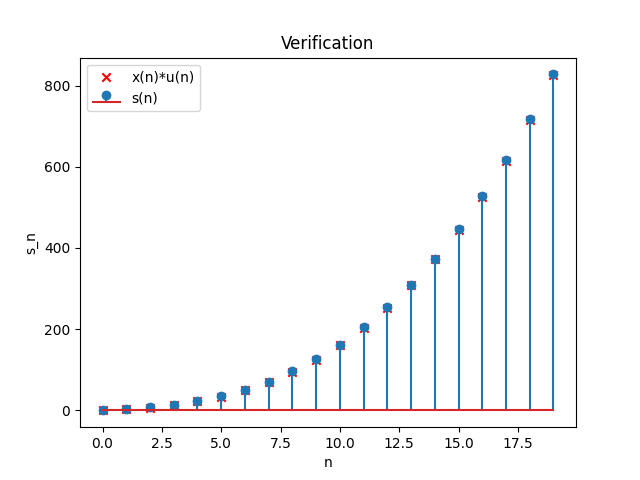
\includegraphics[width=1\columnwidth]{ncert-maths/11/9/5/25/figs/plot.png}
   \caption{Plot of s(n) vs n}
   \label {fig: 11.9.5.25.1}
\end{figure}

